% !TeX program = xelatex
\documentclass[UTF8,a4paper,zihao=-4,fontset=fandol]{ctexart}
\usepackage[left=24mm,right=24mm,top=22mm,bottom=22mm]{geometry}
\usepackage{amsmath,amssymb,booktabs,graphicx,float,array,longtable,enumitem,xcolor,hyperref,listings,tikz}
\usetikzlibrary{arrows.meta,positioning,calc}
\setmainfont{TeX Gyre Termes}
\hypersetup{colorlinks=true,linkcolor=black,urlcolor=blue,citecolor=black}
\ctexset{section={format=\centering\heiti\zihao{4},name={,、},number=\chinese{section},aftername=\quad},subsection={format=\heiti\zihao{-4},number=\arabic{section}.\arabic{subsection},aftername=\quad},subsubsection={format=\heiti\zihao{五号},number=\arabic{section}.\arabic{subsection}.\arabic{subsubsection},aftername=\quad}}
\setlength{\parindent}{2em}\linespread{1.18}\pagestyle{plain}
\setlist{nosep,leftmargin=2em}
\lstset{basicstyle=\ttfamily\scriptsize,breaklines=true,frame=single,columns=fullflexible}
\newcommand{\source}[1]{\par\smallskip\noindent{\footnotesize 数据来源：#1}}
\newcommand{\keywords}[1]{\par\noindent\textbf{关键词：}#1}
\begin{document}
\begin{center}
{\heiti\zihao{2}机器狗对无线电干扰源的定位与清除研究\par}
\vspace{8pt}{\zihao{-4}全国大学生数学建模竞赛 B 题阶段论文稿\par}
\vspace{6pt}{\zihao{-5}匿名版；队号、成员信息和正式测试结果在提交前按官方要求补录\par}
\end{center}
\begin{abstract}
题目要求机器狗在半径 $1800\,\mathrm m$ 的区域内，通过带有测角误差的串行接口寻找并清除数量未知的无线电干扰源。我们把任务写成“有界误差定位—覆盖证书—在线巡回”的组合决策问题。对单源定位，采用测向楔形半平面交，并以外切圆盘保持接收约束；对清除判定，以可能区域的最小包围圆半径不超过 $19.75\,\mathrm m$ 作为带余量的安全证书；对全向源，构造原点加六站覆盖；对未知朝向源，构造 16 点外环、8 点内环和原点组成的 25 站同心环三角覆盖，并用凸组合反证保证至少一个顶点同时满足距离和发射半平面条件。问题 2 在候选点上计算线性化误差代理并加入移动代价，问题 3 采用动态 $q_{10}$ 测向，问题 4 采用覆盖与末端清除联合巡回。50 个共同合成场景中，问题 3 的动态策略为 $333.75\,\mathrm{s/源}$，问题 4 的 25 站联合策略为 $587.22\,\mathrm{s/源}$，均完成全部清除；这些数字是本地验证结果。已有 7 局官方演练共清除 92 个源，验证了接口、计时和完成证书，但不同策略未使用共同隐藏场景，不能替代正式成绩。\par
\keywords{无线电测向；有界误差；最小包围圆；覆盖证明；在线巡回}
\end{abstract}
\newpage
\section{问题重述与任务分析}
\subsection{问题背景}
机器狗携带测向传感器和近距离光学清除装置，从目标区域中心出发，按照接口反馈逐步寻找无线电干扰源。干扰源的位置、频道和总数都不预先公开；一次动作只能针对一个频道和一个位置，接口返回当前频道的 \texttt{direction}、\texttt{near} 或 \texttt{no\_signal}。测向角存在不超过 $1^\circ$ 的误差，机器狗的运动速度为 $5\,\mathrm{m/s}$，测量、换频、移动和清除都计入同一虚拟时钟。源进入 $20\,\mathrm m$ 范围后才能尝试清除，因而“发现了方向”与“已经可以安全清除”是两个不同的停止条件。题目背景和接口约束以竞赛官网公布的规则为准\cite{cumcm}。

本题的困难来自信息的不对称。程序知道自己走过的坐标和接口反馈，却不能读取隐藏源坐标，也不能把一次没有信号解释为频道为空。第三问的源均全向，接收半径决定可见性；第四问的定向源还只在一个未知闭半平面内发射，同一位置换一个测量站可能从有信号变为无信号。策略必须在不知道真值的情况下逐步缩小可能区域，并且在结束前给出覆盖和清除两类可核查证据。

第三问的源均为全向源，重点是用有限站点完成全域发现，再根据多次测向收缩位置区域。第四问增加未知发射方向：检测点即使距离足够近，也可能位于发射半平面之外，因此“无信号”不能直接当作该频道不存在。该变化使覆盖证书和定位策略必须同时考虑。

\subsection{任务的输入、输出与评价}
\begin{table}[H]\centering\small
\caption{题目要求、输出和本文方法}\label{tab:q1-tasks}
\begin{tabular}{p{0.12\linewidth}p{0.35\linewidth}p{0.39\linewidth}}
\toprule
问题 & 输入与约束 & 输出与评价 \\
\midrule
1 & 多个检测位置、示向度和误差界 & 可行定位区域、直径、最小包围圆及一次清除判据 \\
2 & 首次检测位置、示向度及候选移动位置 & 可接收候选集、候选点排序和后验定位误差 \\
3 & 串行反馈、全向源、区域覆盖要求 & 全部源的发现、定位、清除策略及虚拟时间 \\
4 & 问题3信息，加未知源类型和发射方向 & 面向定向盲区的覆盖策略、清除证书和鲁棒性评价 \\
\bottomrule
\end{tabular}
\end{table}

表~\ref{tab:q1-tasks} 中的“输入”均指题目给出的规则和当前接口反馈，而非合成环境中的隐藏真值。程序把每个动作的请求、响应和虚拟时钟写入逐动作日志；论文中的数值只从这些日志或固定种子合成运行中读取。评价先看是否完成覆盖并清除全部源，再比较虚拟时间；若两者冲突，完整性优先。反馈驱动的决策循环见图~\ref{fig:q1-workflow}。

\subsection{建模主线}
我们将每个频道的状态写成 $(\mathcal P_k,\,z_k,\,c_k)$：$\mathcal P_k$ 是由已有反馈保留下来的可能位置集合，$z_k$ 表示是否已发现，$c_k$ 表示是否已清除。一次 \texttt{direction} 反馈把一个带角度误差的楔形约束加入 $\mathcal P_k$；\texttt{near} 直接触发同位置清除；\texttt{no\_signal} 只更新测量记录，不擅自删除候选位置。每一次动作先通过协议客户端取得反馈，再更新对应状态，策略不读取隐藏源坐标。

决策目标按词典序排列：先满足覆盖和清除证书，再比较总虚拟时间、移动距离、测量次数和兜底次数。问题四的覆盖阶段和末端阶段因此承担不同任务：前者完成对未知朝向的发现证书并积累方向信息，后者在可能区域已经收缩后集中清除。这样的排序避免把“较快但漏源”的结果误当成优解，也为后面的算法比较提供统一口径。

\begin{figure}[H]\centering
\begin{tikzpicture}[>=Latex,node distance=10mm]
\node[draw,rounded corners,fill=gray!10,minimum width=30mm,minimum height=9mm] (a) {题面/接口反馈};
\node[draw,rounded corners,fill=gray!10,minimum width=30mm,minimum height=9mm,right=of a] (b) {集合状态更新};
\node[draw,rounded corners,fill=gray!10,minimum width=30mm,minimum height=9mm,right=of b] (c) {下一停靠点};
\node[draw,rounded corners,fill=gray!10,minimum width=30mm,minimum height=9mm,right=of c] (d) {清除证书};
\draw[->] (a)--(b);\draw[->] (b)--(c);\draw[->] (c)--(d);\draw[->,rounded corners] (d) |- ++(0,-12mm) -| (a);
\end{tikzpicture}
\caption{反馈驱动的在线决策循环}\label{fig:q1-workflow}
\source{本文算法流程；不含隐藏真值。}
\end{figure}

\section{问题分析与数据边界}
\subsection{几何信息的保守表达}
若检测点为 $p_i=(x_i,y_i)$、示向度为 $\theta_i$，则真实源点 $g$ 位于以 $p_i$ 为顶点、方向 $\theta_i$ 为中心的误差楔形内。将每个楔形写成两个线性不等式后，多次观测的交集仍为凸集。接收半径 $R\in[1000,1500]\,\mathrm m$ 形成圆盘边界；实现以外切正多边形包围圆盘，宁可保留少量不可能点，也不因离散化排除真实点。

\subsection{时间和风险的分解}
题面虚拟时间按
\begin{equation}\label{eq:time}
T=\frac{L}{5}+N_{\rm sw}+5N_{\rm mea}+3N_{\rm clr}+2N_{\rm suc}
\end{equation}
计算，其中 $L$ 为移动距离。移动项通常远大于一次测量项，因此候选点不只追求几何收缩，还要惩罚绕行。另一方面，覆盖站和频道排查构成与源数量无关的固定开销，比较不同样本时不能只看 $T/N$。

\subsection{实验设计与证据等级}
本稿将证据分为三层。第一层是题面和几何推导，支撑“不会漏掉”的条件；第二层是 50 个共同源配置的本地合成配对实验，支撑策略间相对比较；第三层是用户在官方模拟器中手动选择演练得到的 7 局记录，支撑接口、计时、日志和完成证书。正式测试数据目前为空，表格中以“待替换”保留位置。所有本地随机场景、固定种子和官方演练均不写成正式成绩。

\begin{figure}[H]\centering
\begin{tikzpicture}[x=1cm,y=1cm]
\draw[->] (-3.4,0)--(3.6,0) node[right] {$x$};\draw[->] (0,-2.9)--(0,3.1) node[above] {$y$};
\draw (0,0) circle (2.3);\draw[thick,->] (0,0)--(1.7,1.15) node[midway,above] {$\theta_i$};
\draw[red!70!black,thick] (1.7,1.15)--(3.0,2.0);\draw[red!70!black,thick] (1.7,1.15)--(2.9,0.3);
\draw[dashed] (0,0)--(2.3,0) node[midway,below] {$R$};\fill (1.7,1.15) circle (2pt) node[above right] {$p_i$};
\node at (0,-2.55) {测向楔形与接收圆盘的外包};
\end{tikzpicture}
\caption{单次测向反馈的几何约束}\label{fig:wedge}
\source{根据题面误差界绘制；坐标仅作示意。}
\end{figure}

\section{模型假设}
\begin{enumerate}
\item 干扰源在一次任务期间静止，且位置位于半径 $1800\,\mathrm m$ 的目标圆域内；不同频道至多对应一个源。
\item 测向误差的绝对值不超过 $1^\circ$。接口保留两位小数，为覆盖舍入边界，程序内部使用 $\varepsilon_{\rm api}=1.01^\circ$。
\item 当检测点与源距离不超过 $20\,\mathrm m$ 时，光学装置可以完成清除；因此定位算法必须保证可能区域整体落入该半径，而不能只使用点估计。
\item 机器狗按串行接口执行动作；动作返回未被接受时，不推进本地位置和虚拟时间。网络重试沿用同一请求标识，不并发发送动作。
\end{enumerate}

以上假设直接服务于题面规则。圆盘外切多边形的边数、候选角度间隔、路程权重和覆盖网格属于算法参数，不当作物理事实。合成实验采用圆域均匀源位置、$N\in\{10,\ldots,16\}$ 和频道无放回抽样，仅用于可重复比较；官方模拟器的隐藏分布未知。

\begin{figure}[H]\centering
\begin{tikzpicture}[>=Latex]
\node[draw,rounded corners,fill=blue!8,minimum width=31mm,minimum height=9mm] (a) at (0,0) {题面事实};
\node[draw,rounded corners,fill=green!8,minimum width=31mm,minimum height=9mm] (b) at (4,0) {实现参数};
\node[draw,rounded corners,fill=orange!12,minimum width=31mm,minimum height=9mm] (c) at (2,-1.6) {实验分布};
\draw[->] (a)--(b) node[midway,above] {固定约束};\draw[->] (a)--(c);\draw[->] (b)--(c) node[midway,right] {仅用于比较};
\end{tikzpicture}
\caption{假设、实现参数和实验分布的边界}\label{fig:assumption}
\source{本文分层记录。}
\end{figure}

\section{符号说明}
\begin{longtable}{p{0.2\linewidth}p{0.68\linewidth}}
\caption{主要符号及含义}\label{tab:q1-notation}\\
\toprule 符号 & 含义 \\
\midrule\endfirsthead
\toprule 符号 & 含义 \\
\midrule\endhead
$\Omega$ & 半径 $1800\,\mathrm m$ 的目标圆域 \\
$g,p_i$ & 源位置、 第 $i$ 个检测位置 \\
$\theta_i,\varepsilon$ & 示向度、测向误差界 \\
$W_i$ & 第 $i$ 次测量的误差楔形 \\
$\mathcal P_k$ & 频道 $k$ 当前可能位置集合 \\
$D(\mathcal P)$ & 可能区域直径 \\
$(c^*,R^*)$ & 可能区域的最小包围圆圆心和半径 \\
$L,N_{\rm sw},N_{\rm mea}$ & 总路程、换频次数、测量次数 \\
$N_{\rm clr},N_{\rm suc}$ & 清除尝试次数、成功次数 \\
$U(q,g)$ & 候选测点 $q$ 在假定位置 $g$ 下的线性化误差代理 \\
$\lambda$ & 移动距离权重 \\
$r_o,r_i$ & 问题四外环、内环半径 \\
$n_s,n_m,n_c,n_f$ & 站点、测量、清除和光学兜底动作计数 \\
$T_{\rm move},T_{\rm mea},T_{\rm clr}$ & 移动、测量和清除对应的虚拟时间分量 \\
\bottomrule
\end{longtable}

表~\ref{tab:q1-notation} 中的符号贯穿四个子问题；其中 $\mathcal P_k$ 和 $R^*$ 是从测量反馈到安全清除判定的主要状态量。

\section{问题一：有界测角误差下的定位区域}
\subsection{半平面交模型}
令 $u(\theta)=(\cos\theta,\sin\theta)$，二维叉积记为 $\operatorname{cross}(a,b)=a_xb_y-a_yb_x$。第 $i$ 次观测的可行楔形写成
\begin{equation}\label{eq:wedge}
W_i=\{g:\operatorname{cross}(u(\theta_i-\varepsilon),g-p_i)\ge0,\quad \operatorname{cross}(u(\theta_i+\varepsilon),g-p_i)\le0\}.
\end{equation}
将式 \eqref{eq:wedge} 改写为 $A_i g\le b_i$，即可用线性规划检查空集和无界性；有界时枚举约束直线交点，再取凸包得到 $\mathcal P=\cap_iW_i$。与人为设置一个大正方形相比，该做法能明确返回 EMPTY、UNBOUNDED 或 BOUNDED 三种状态。

考虑接收区域时，程序将半径 $R$ 的圆盘替换为外切正 $K$ 边形，默认 $K=128$。其最大径向膨胀为 $R(\sec(\pi/K)-1)$，所以所得区域是安全外包，不把外包直径误写成曲边区域的精确直径。

\subsection{直径与最小包围圆}
对凸多边形顶点按逆时针排列，直径由一对对踵点取得，使用旋转卡壳计算；同时用顶点对穷举作独立数值对照。最小包围圆采用随机增量算法，再遍历全部顶点复核包含性，这两个几何子程序分别对应旋转卡壳和最小包围圆的经典做法\cite{toussaint,welzl}。只有
\begin{equation}\label{eq:clear-cert}
R^*(\mathcal P_{\rm out})\le 19.75\,\mathrm m
\end{equation}
时才向圆心发出清除请求，$0.25\,\mathrm m$ 用于数值余量。

\subsection{求解步骤与数值核验}
实现先将所有楔形边界和接收圆盘外切多边形统一写成半平面约束，再枚举约束直线交点。落在全部半平面内的交点按极角排序形成凸多边形；若交点不足以形成有界区域，则分别返回空集或无界状态，不进入清除流程。对有界多边形，旋转卡壳给出直径，随机增量算法给出最小包围圆，并用“所有顶点到圆心的距离不超过半径”作最后复核。该流程把数值几何、清除判定和协议动作分开，便于定位误差来源。

\begin{table}[H]\centering\small
\caption{问题一构造数据的逐步收缩核验}\label{tab:q1-shrink}
\begin{tabular}{rrrr}
\toprule
累计检测点数 & 外包面积 ($\mathrm m^2$) & MEC 半径 ($\mathrm m$) & 清除判定 \\
\midrule
1 & 39279.93 & 750.23 & 否 \\
2 & 2092.03 & 42.56 & 否 \\
3 & 658.61 & 22.52 & 否 \\
\bottomrule
\end{tabular}
\source{results/synthetic/q1.json；由相同构造数据逐次加入观测得到。}
\end{table}

表 \ref{tab:q1-shrink} 中第三次观测已经把区域直径压到 $39.00\,\mathrm m$，但最小包围圆半径仍为 $22.52\,\mathrm m$，因此按照式 \eqref{eq:clear-cert} 不应直接清除。对偶指标的同时记录避免了将“区域面积变小”误作“满足光学距离证书”；完整收缩过程见图~\ref{fig:q1-shrink}。

\begin{figure}[H]\centering
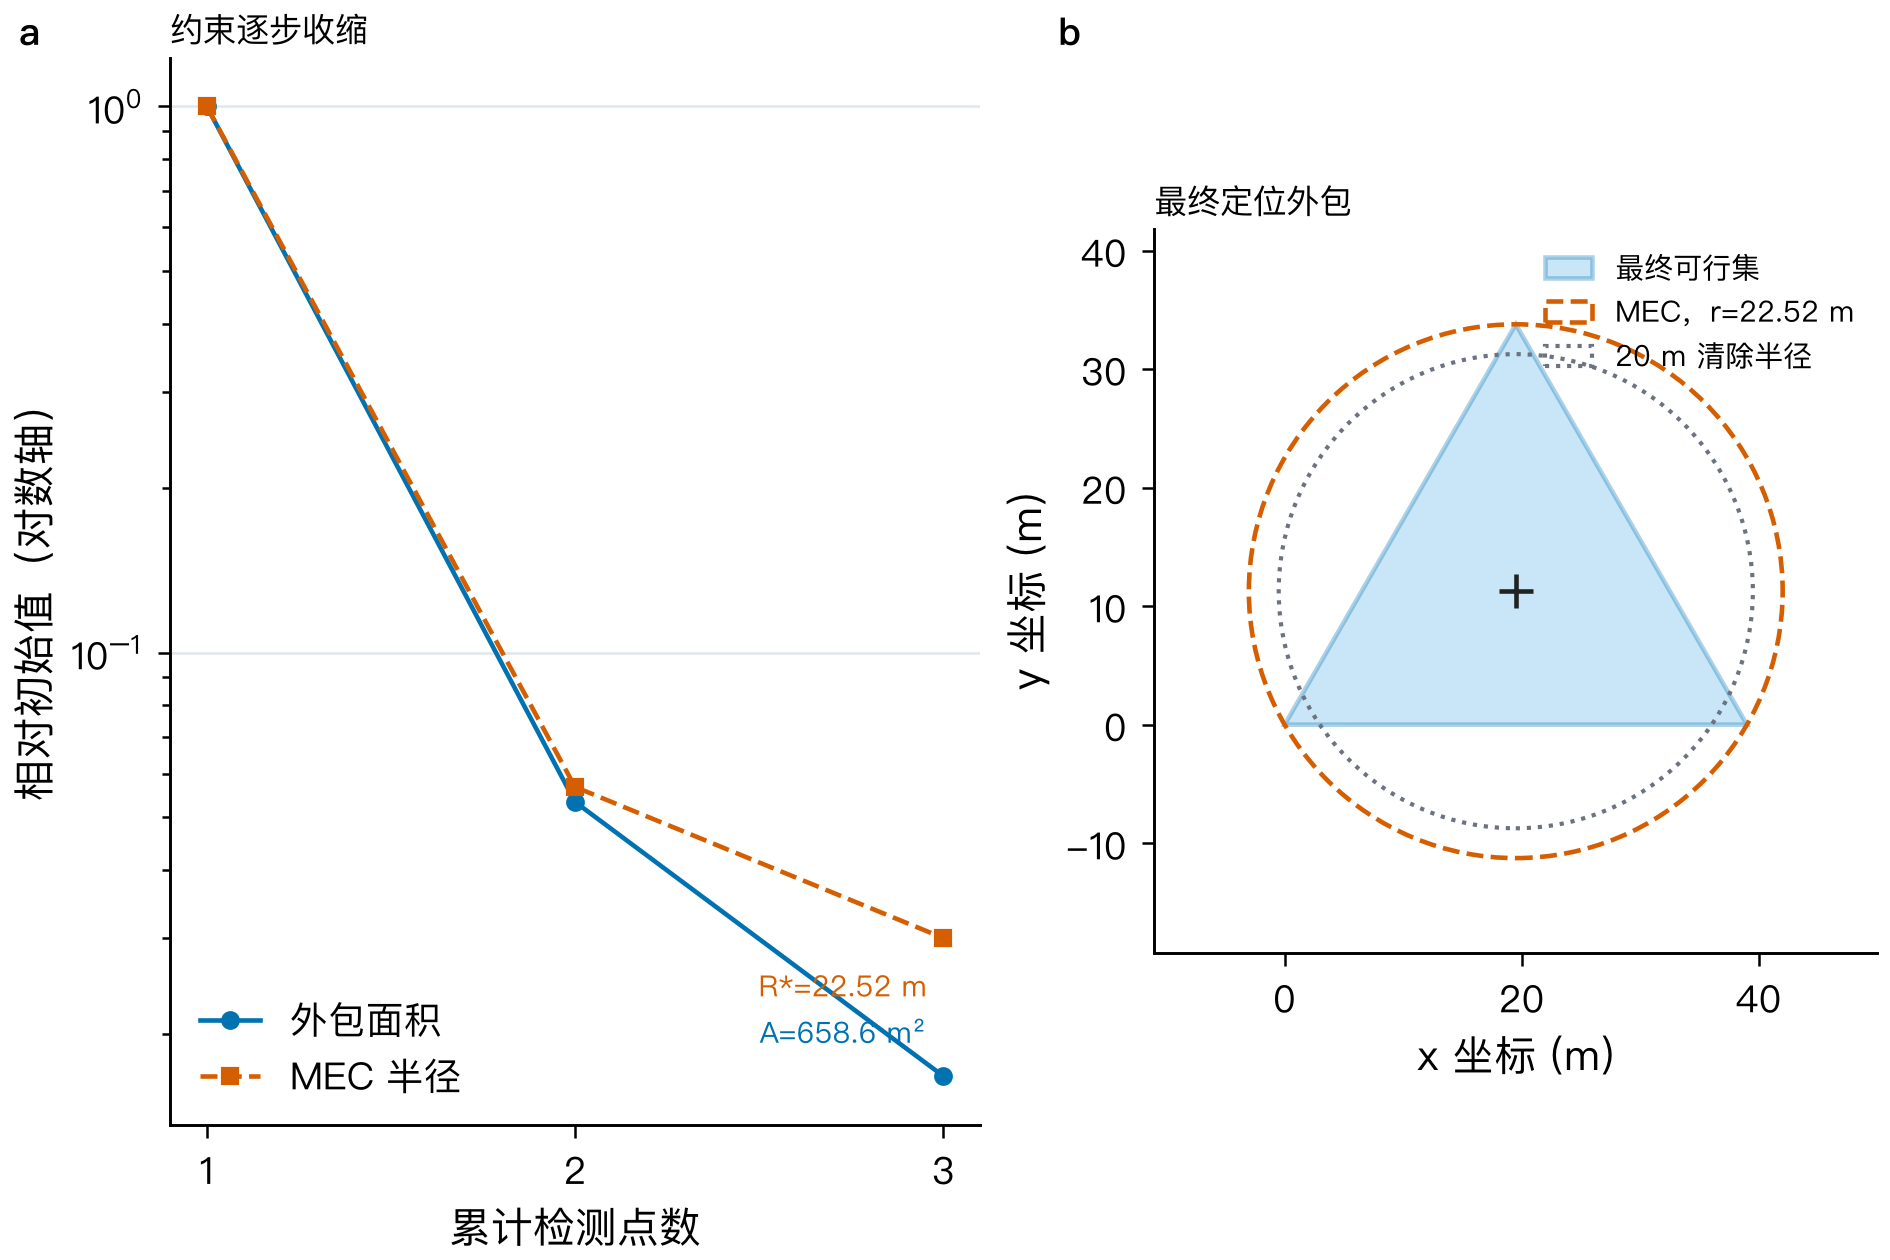
\includegraphics[width=0.98\linewidth]{figures/process_q1_intersection.png}
\caption{测向约束收缩过程与最终清除阈值核对}\label{fig:q1-shrink}
\source{results/synthetic/q1.json；左图为归一化收缩曲线，右图为最终可能区域与包围圆。}
\end{figure}

\subsection{“直径不超过40米”不是充分条件}
构造边长 $39\,\mathrm m$ 的等边三角形。其直径为 $39\,\mathrm m$，而最小包围圆半径为
\begin{equation}
R^*=\frac{39}{\sqrt3}=22.5167\,\mathrm m>20\,\mathrm m.
\end{equation}
因此直径上限不能替代最小包围圆判据。该反例也说明，清除判定必须针对整体可能区域，而不是将多次测向的交会点取平均。

图~\ref{fig:q1-counter} 用同一反例显示两种判据的差别；图~\ref{fig:q1-mec} 则给出多次楔形交集与最小包围圆的几何示意。

\begin{figure}[H]\centering
\begin{tikzpicture}[scale=0.08]
\coordinate (A) at (0,0);\coordinate (B) at (39,0);\coordinate (C) at (19.5,33.775);
\draw[thick] (A)--(B)--(C)--cycle;\draw[dashed] (19.5,11.258) circle (22.517);
\fill (19.5,11.258) circle (1.1);\draw[<->] (A)--(B) node[midway,below] {$39\,\mathrm m$};
\node at (19.5,-9) {直径 $39$ 米，但包围圆半径 $22.52$ 米};
\end{tikzpicture}
\caption{问题一的等边三角形反例}\label{fig:q1-counter}
\source{构造数据，数值来自 results/synthetic/q1.json。}
\end{figure}

\begin{figure}[H]\centering
\begin{tikzpicture}[x=1cm,y=1cm]
\draw[gray!60] (-3,-2.2) rectangle (3.2,2.4);\draw[thick] (-2.5,-1.5)--(2.4,-1.5)--(1.0,1.8)--cycle;
\draw[dashed] (0.0,0.1) circle (1.35);\fill (0,0.1) circle (1.5pt);
\node at (0,-2.7) {楔形交集 $\mathcal P$ 与最小包围圆};
\end{tikzpicture}
\caption{多次测向逐步收缩可能区域的示意}\label{fig:q1-mec}
\source{几何示意图；实际算法使用外切圆盘和凸多边形顶点。}
\end{figure}

\section{问题二：主动测向点的选择}
\subsection{可接收候选集}
首次观测得到外包区域 $\mathcal P_1$ 后，若希望对全向源保留接收保证，候选点 $q$ 应满足 $\max_{g\in\mathcal P_1}\|q-g\|\le1000$。因为距离函数对 $g$ 是凸函数，最大值在凸多边形顶点取得，故可用
\begin{equation}\label{eq:safe}
\mathcal C_{\rm safe}=\bigcap_{v\in\operatorname{vert}(\mathcal P_1)}B(v,1000)
\end{equation}
离散构造候选集。若该集合为空，程序保留风险标记并继续做后验核验，不把离散空集解释成物理不可能。

\subsection{几何误差代理与移动惩罚}
在假定源位置 $g$ 下，角度观测的雅可比行为向量为
\begin{equation}
h_i(g)=\frac{1}{\|g-p_i\|^2}\bigl(-(g_y-p_{iy}),\;g_x-p_{ix}\bigr).
\end{equation}
将已有观测和候选观测组成矩阵 $H$，用 $H^+$ 估计角度盒误差引起的位置扰动，定义
\begin{equation}\label{eq:score}
U(q,g)=\varepsilon_{\rm api}\sum_j\|H^+_{:,j}\|_2,\qquad
S(q)=Q_{\alpha}\{U(q,g):g\in\mathcal G\}+\lambda\|q-p_{\rm cur}\|.
\end{equation}
其中 $\mathcal G$ 由外包多边形顶点、边中点、中心和近边界采样组成。$U$ 只用于排序，最终清除仍由式 \eqref{eq:clear-cert} 认证。

当前策略在首次主动点使用较大移动权重，先获取第二条独立几何约束；后续阶段使用 $\alpha=0.10$ 的分位数目标和 $\lambda=0.02$。作为消融，保留最坏值、$\alpha=0.25$、中位数和更细角度候选。

\begin{figure}[H]\centering
\begin{tikzpicture}[x=1cm,y=1cm]
\draw[gray!50] (-3,-2.2) rectangle (3.2,2.3);\draw[thick] (-2.3,-1.3)--(1.9,-1.3)--(1.0,1.5)--cycle;
\fill (0.2,0.0) circle (2pt) node[below right] {$p_{\rm cur}$};
\foreach \a/\lab in {20/A,80/B,140/C,200/D,260/E,320/F}{\fill ({1.6*cos(\a)},{1.6*sin(\a)}) circle (1.4pt) node[above right] {\lab};}
\draw[->,blue] (0.2,0)--(1.6,0.58) node[midway,above] {$S(q)$};
\node at (0,-2.65) {候选点同时受接收、信息和路程约束};
\end{tikzpicture}
\caption{问题二候选点的筛选与排序示意}\label{fig:q2candidate}
\source{候选生成逻辑；点位为示意。}
\end{figure}

\section{问题三：全向源的覆盖与在线清除}
\subsection{七站全域发现证书}
取原点和半径 $a=900\sqrt3\,\mathrm m$、方位角 $0^\circ,60^\circ,\ldots,300^\circ$ 的六个外围站。对任意源点 $g$，若 $\|g\|\le900$，原点距其不超过 $900$；否则选择与 $g$ 夹角不超过 $30^\circ$ 的外围站。距离平方为 $r^2+a^2-2ar\cos\alpha$，在 $r\in[900,1800]$、$\alpha\le30^\circ$ 上的最大值为 $900^2$。故至少一个站点距源不超过 $900\,\mathrm m<1000\,\mathrm m$，扫描七站可以发现全向源。

\begin{figure}[H]\centering
\begin{tikzpicture}[x=1cm,y=1cm]
\draw[thick] (0,0) circle (2.2);\foreach \a in {0,60,120,180,240,300}{\fill ({2.0*cos(\a)},{2.0*sin(\a)}) circle (2pt);}
\fill (0,0) circle (2pt);\foreach \a/\b in {0/1,60/2,120/3,180/4,240/5,300/6}{\node at ({2.25*cos(\a)},{2.25*sin(\a)}) {\b};}
\fill[red] (0.65,1.25) circle (2pt) node[above right] {源};\draw[dashed] (0.65,1.25)--(1,1.732);
\node at (0,-2.65) {原点加六站的全向覆盖};
\end{tikzpicture}
\caption{问题三七站覆盖构造}\label{fig:q3stations}
\source{理论构造；比例仅作示意。}
\end{figure}

\subsection{在线策略}
每个频道维护观测列表、外包可能区域和清除状态。到达站点后，先测量尚未被证明不存在的频道；$\texttt{no\_signal}$ 不直接删除频道。对已有方向反馈的频道，按当前最小包围圆半径保留最多四个测向名额，优先处理不确定性最大的频道。定位达到式 \eqref{eq:clear-cert} 后立即清除；最多连续六次主动测向仍未收敛时，转入 $25\,\mathrm m$ 光学方格兜底。

默认入口为 `adaptive\_q10\_dynamic`：刚发现频道的第一处主动点提高移动惩罚，之后转向 $q_{10}$ 信息目标。七站全部访问且所有已发现频道已清除后，才根据频道上界和覆盖证书退出。

\begin{figure}[H]\centering
\begin{tikzpicture}[>=Latex,node distance=8mm]
\node[draw,rounded corners] (a) {站点扫描};\node[draw,rounded corners,right=of a] (b) {楔形更新};\node[draw,rounded corners,right=of b] (c) {MEC判定};\node[draw,rounded corners,right=of c] (d) {清除/兜底};
\draw[->] (a)--(b);\draw[->] (b)--(c);\draw[->] (c)--(d);\draw[->,rounded corners] (d) |- ++(0,-9mm) -| (a);
\end{tikzpicture}
\caption{问题三在线状态机}\label{fig:q3state}
\source{策略伪流程。}
\end{figure}

\section{问题四：未知朝向源的覆盖与联合巡回}
\subsection{定向盲区的覆盖证书}
未知朝向意味着接收条件除距离外还要求检测点位于源发射方向的闭半平面内。本轮采用 \texttt{ring25} 同心环三角剖分：外环 16 点位于半径 $1800/\cos(\pi/16)+1\,\mathrm m$ 的正十六边形，内环 8 点位于半径 $997\,\mathrm m$ 的正八边形，再补入原点，共 25 个站点。每个 $45^\circ$ 扇区拆成三个三角形，内环区域拆成八个三角形；代码检查每个单元的最大边长不超过 $1000\,\mathrm m$，外环切线距离覆盖 $1800\,\mathrm m$ 圆盘。

设发射方向单位向量为 $d$。若某个覆盖三角形的三个顶点均满足 $d\cdot(p_j-g)<0$，则对包含 $g$ 的凸组合加权会得到 $d\cdot(g-g)<0$，矛盾。因此至少一个顶点满足闭半平面条件。该证明同时覆盖边界点、向外发射方向和源位于网格顶点的情形；外环额外留出的 1 m 只用于抵抗边界浮点舍入。

从几何上看，外环半径取 $r_o=1800/\cos(\pi/16)+1\,\mathrm m$，即在外接半径基础上增加 $1\,\mathrm m$，对应切向余量约 $0.981\,\mathrm m$；内环半径取 $r_i=997\,\mathrm m$，使中心三角形和外侧三角形的最长边均处于 1000 m 接收半径以内。程序对 32 个三角形逐一计算三条边长，并用随机圆盘点与等角圆周点做包含性采样。该数值检查是对解析证书的独立实现核对，不能替代解析证明，也不把抽样通过写成对连续域的额外定理。

环形站点和访问编号见图~\ref{fig:q4-coverage}；图中的三角形是覆盖证书单元，折线才是机器狗的站点访问路线，两者用途不同。

\begin{figure}[H]\centering
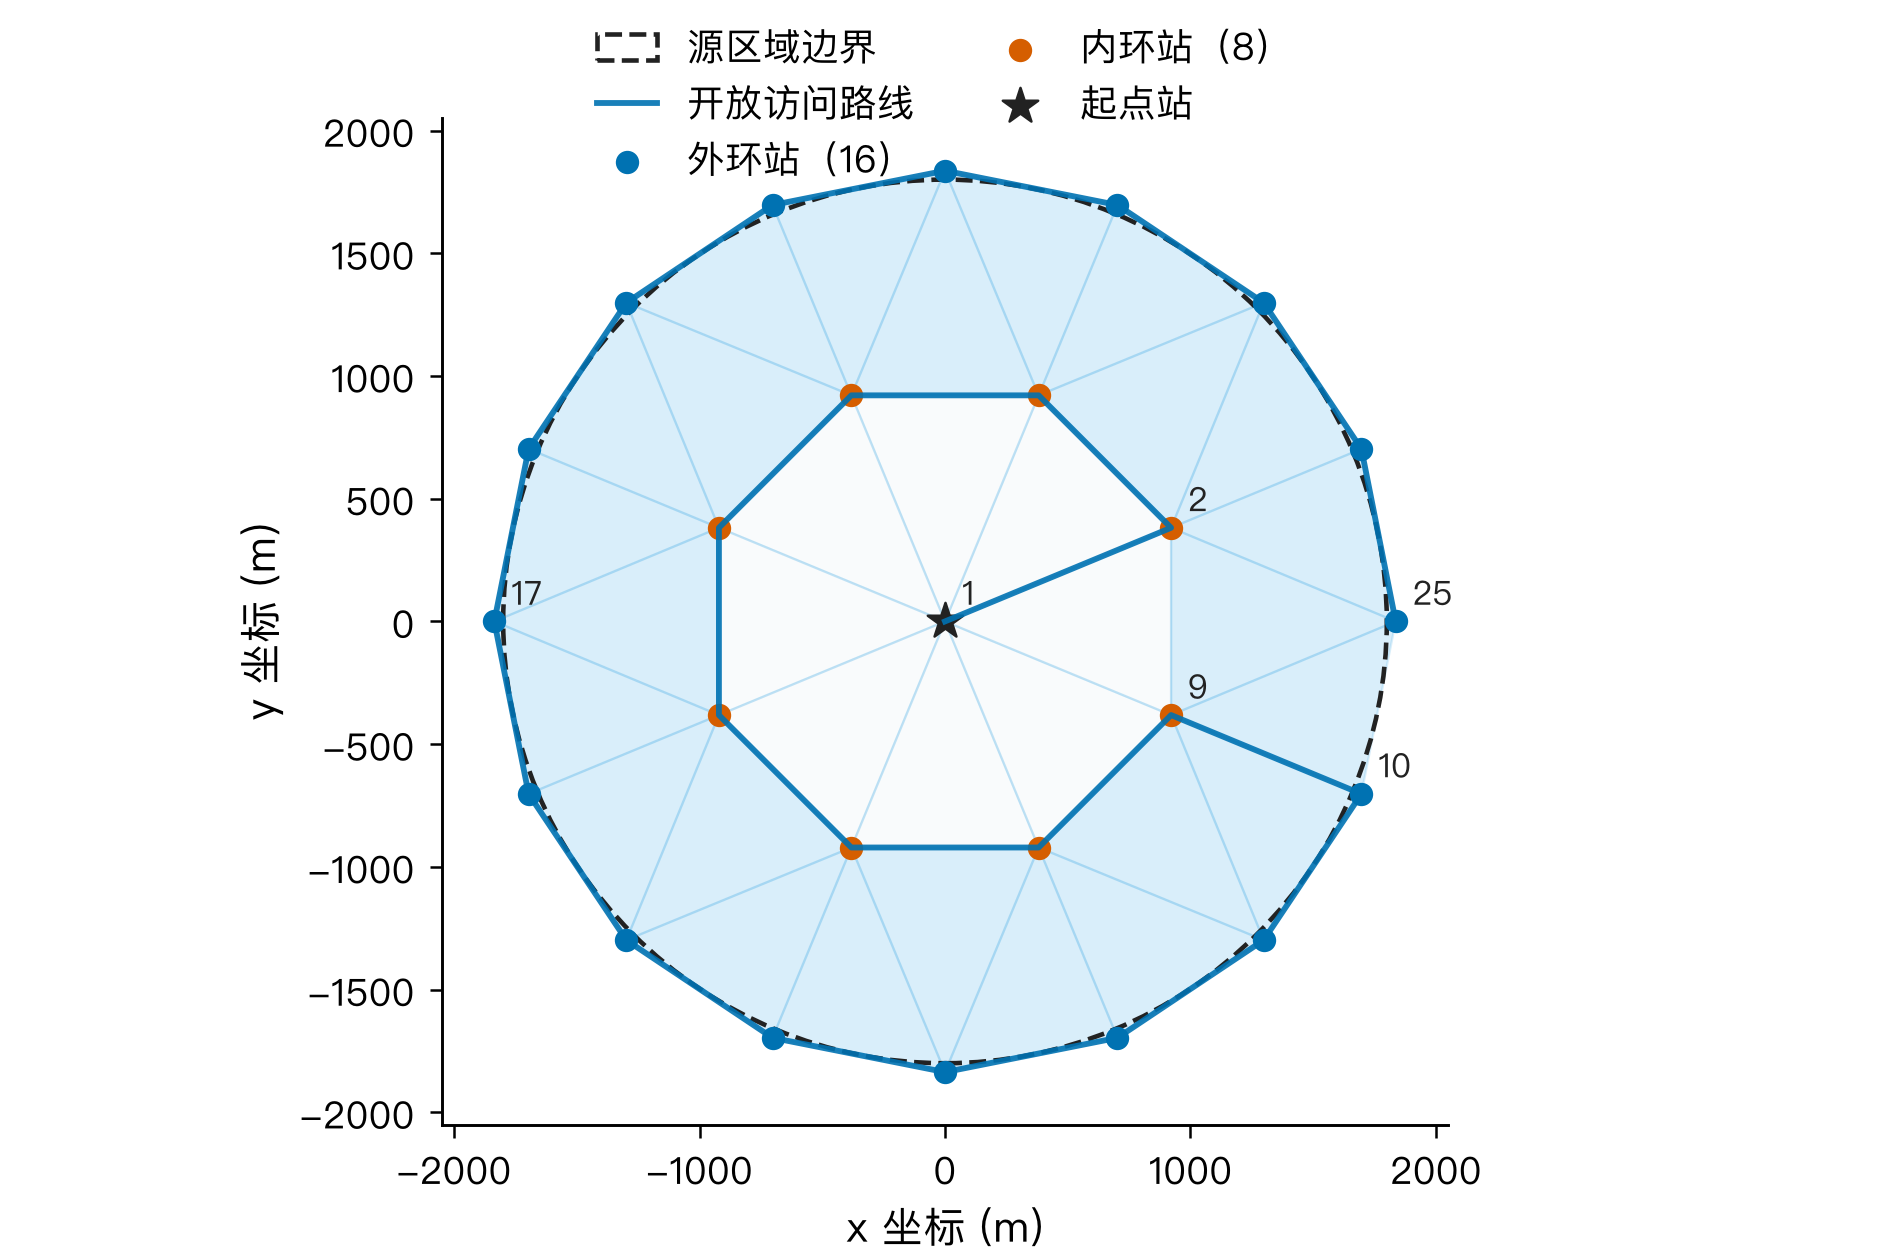
\includegraphics[width=0.82\linewidth]{figures/process_q4_coverage.png}
\caption{问题四的 25 站同心环三角覆盖与开放访问路线}\label{fig:q4-coverage}
\source{ring25_cover 的确定性构造；32 个覆盖单元，图中编号为访问顺序。}
\end{figure}

将站点集合记为 $P=\{p_0,\ldots,p_{n-1}\}$，开放访问路线 $\pi$ 的几何长度为
\begin{equation}
L_{\rm station}(\pi)=\|p_0-p_{\pi_1}\|+\sum_{i=2}^{n-1}\|p_{\pi_i}-p_{\pi_{i-1}}\|.
\end{equation}
当前实现先用最近邻生成可行顺序，再用 2-opt 反转子段；它只优化覆盖站之间的开放路径，不改变覆盖单元或清除判据。由同一段代码直接复核，25 站环形路线的站点长度为 $17{,}924.88\,\mathrm m$，26 站三角路线为 $24{,}078.75\,\mathrm m$，具体数值见表~\ref{tab:q4-route-length}。该长度不包含逐频道测量和末端目标清除的移动。

\begin{table}[H]\centering\small
\caption{覆盖站开放路线的几何长度核验}\label{tab:q4-route-length}
\begin{tabular}{lrrr}
\toprule
覆盖构造 & 站点数 & $L_{\rm station}$ (m) & 相对 26 站三角 \\
\midrule
26 站三角 & 26 & 24078.75 & 基线 \\
25 站环形 & 25 & 17924.88 & -25.56\% \\
\bottomrule
\end{tabular}
\source{src/cumcm\_b/policy.py 的 q4\_station\_route；确定性几何计算。}
\end{table}

\subsection{联合巡回策略}
覆盖阶段按固定开路径访问 25 个站点，对未知频道逐站扫描；对已有方向频道只保留最多三个当前最小包围圆半径最大的补充测向，默认不在巡回中触发光学方格。覆盖结束后，将所有已发现频道的当前包围圆圆心作为目标点，采用最近邻初始化、开放路径 2-opt 改善访问顺序，逐目标执行安全清除或有限兜底。这样的“覆盖单元—路线—末端处理”分层与公开覆盖规划库的模块化思路一致\cite{fields2cover,opennav,coverage}；有限测量名额按当前可能区域半径排序，优先处理不确定性最大的频道，滚动 q10 信息目标则在末端定位阶段执行。覆盖引导图、有限视界收益评估以及信息路径规划中的节点奖励思想分别可见 CAP、adaptive coverage、AIPP 与 SISL 的公开工作\cite{cap,adaptivecoverage,aipp,sisl}；本文只借鉴其分层与收益排序思想，清除安全仍由闭集几何证书决定。该分阶段设计还来自官方演练日志：同一未收敛频道在多个站点重复清除会产生大量无效请求。

联合目标可以写成词典序问题：首先要求所有覆盖站访问完毕且 $c_k=1$ 对所有已发现频道成立；在可行解集合内，再最小化 $T$。覆盖阶段的固定路线使几何证书与移动路线可独立复核，末端阶段的 2-opt 只改变目标访问顺序，不改变每个频道的 $R^*$ 判据。若当前目标仍未满足清除证书，算法最多进行规定次数的主动测向，随后调用与可能区域相交的光学方格；因此路线优化不会以牺牲清除安全性为代价。

图~\ref{fig:q4-route} 是两阶段策略的抽象流程，图~\ref{fig:q4-trajectory} 则把同一思想映射到过程日志中的实际动作和虚拟时间。

\begin{figure}[H]\centering
\begin{tikzpicture}[x=1cm,y=1cm]
\draw[thick,rounded corners] (-3,-1.9) rectangle (3.2,2.0);\draw[step=0.9,gray!40] (-2.8,-1.7) grid (3,1.8);
\draw[very thick,blue,->] (-2.4,-1.3)--(-1.2,0.8)--(0.0,-1.2)--(1.1,1.3)--(2.6,-0.8);
\foreach \p in {(-2.4,-1.3),(-1.2,0.8),(0,-1.2),(1.1,1.3),(2.6,-0.8)}{\fill \p circle (2pt);}
\node at (0,-2.35) {覆盖阶段收集信息，末端阶段清除目标};
\end{tikzpicture}
\caption{问题四两阶段联合巡回示意}\label{fig:q4-route}
\source{路径结构示意；真实站点坐标由程序生成。}
\end{figure}

\begin{figure}[H]\centering
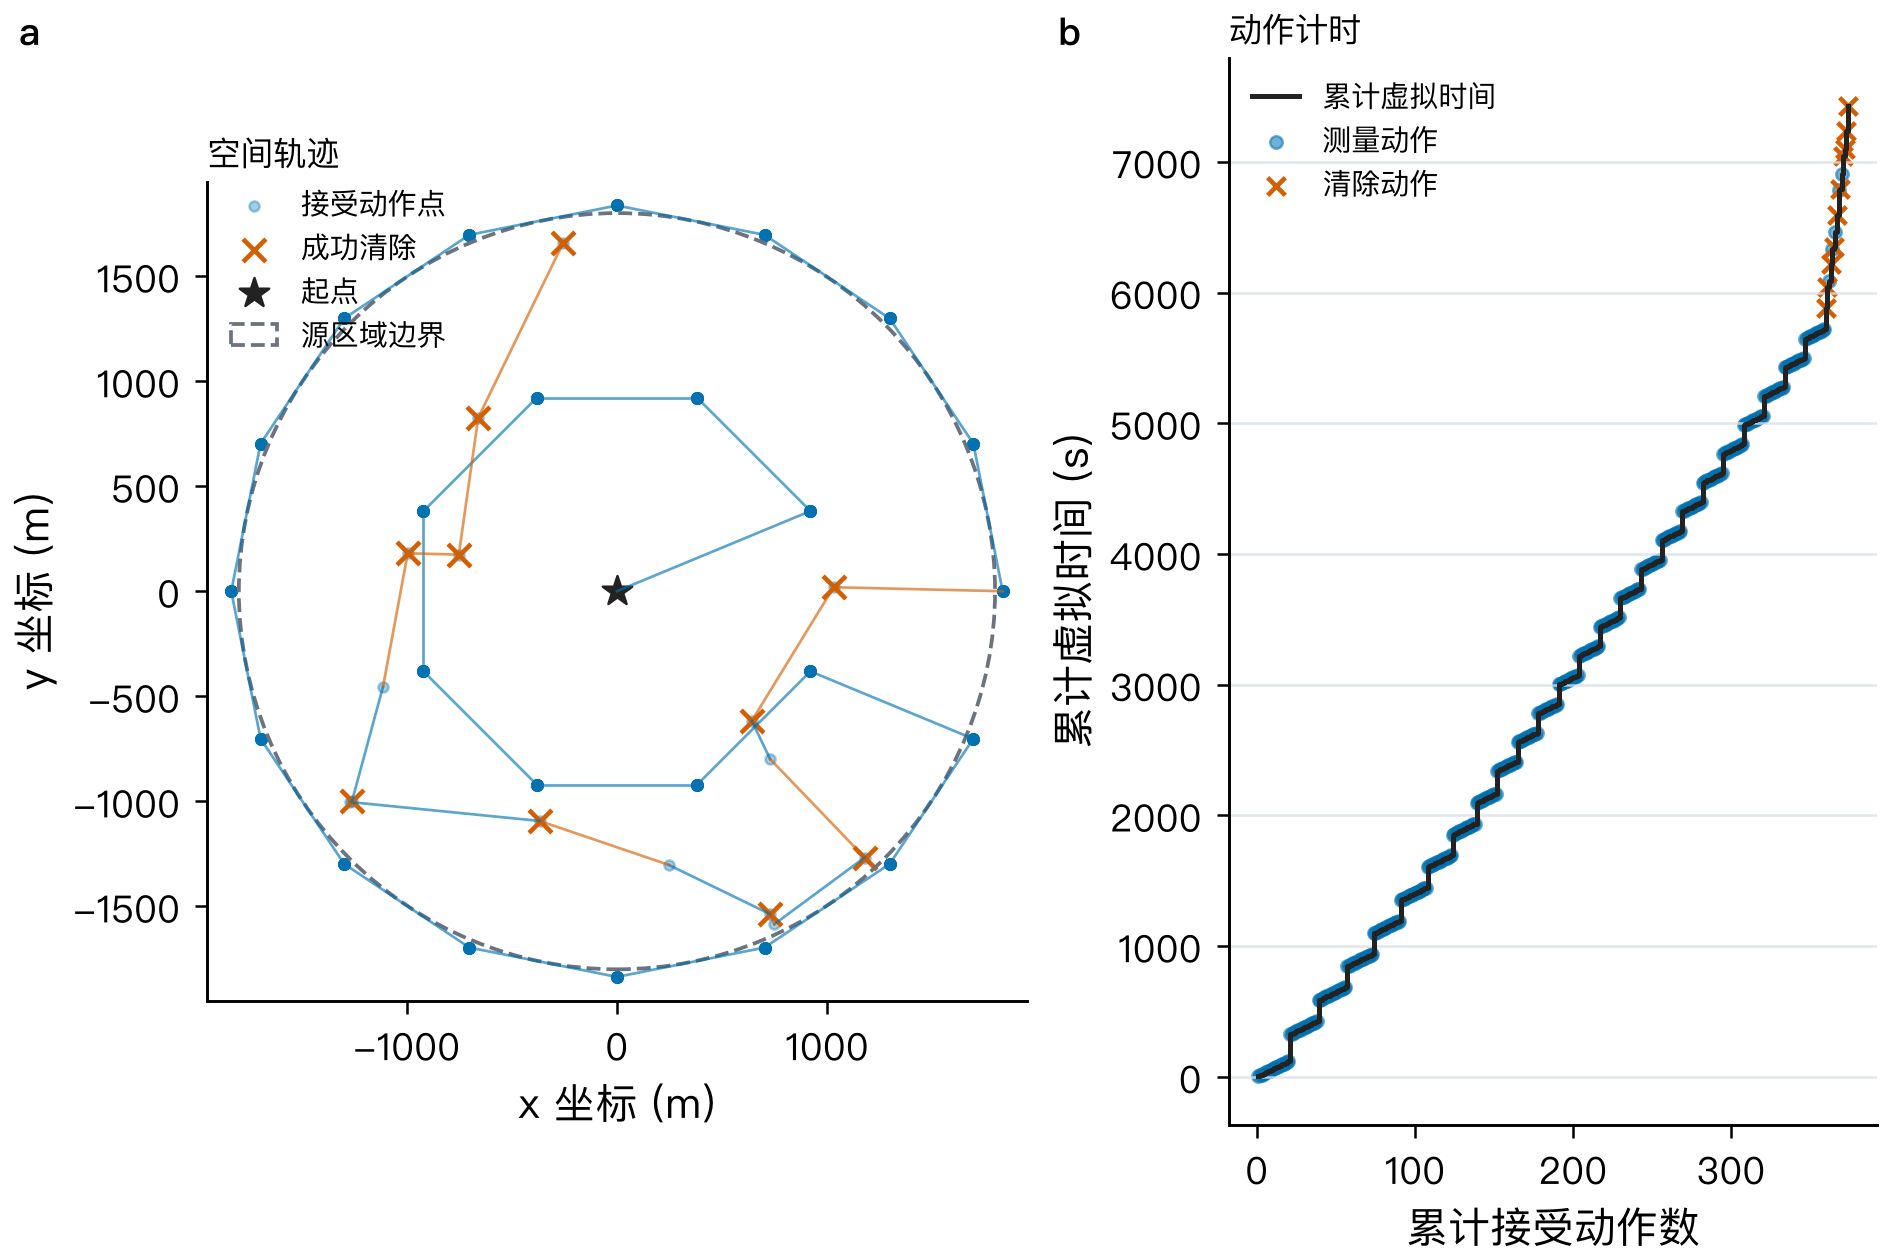
\includegraphics[width=0.98\linewidth]{figures/process_q4_trajectory.png}
\caption{问题四过程记录中的空间轨迹与累计虚拟时间}\label{fig:q4-trajectory}
\source{results/synthetic/q4_current_trace.json；q4\_joint，ring25，种子 20260911，本地合成过程记录。}
\end{figure}

\section{实验结果、敏感性与模型评价}
\subsection{问题一与问题二的数值核验}
问题一构造数据得到三角形直径 $39.0000\,\mathrm m$、穷举直径 $39.0000\,\mathrm m$、最小包围圆半径 $22.5167\,\mathrm m$，与理论推导一致。问题二在 6 个源距、3 个首次误差和 3 个第二次误差组合下进行后验核验，全部候选点可接收；例如源距 $600\,\mathrm m$ 时后验半径约为 $16.48$--$16.71\,\mathrm m$，源距 $1200\,\mathrm m$ 时约为 $38.15$--$44.16\,\mathrm m$。这说明远距离测向的几何退化会直接反映到候选点排序中。

\subsection{问题三与问题四的配对结果}
\begin{table}[H]\centering\small
\caption{共同合成场景的策略比较}\label{tab:paired}
\begin{tabular}{lrrrrr}
\toprule
方案 & 场景数 & 平均秒/源 & 平均路程(m) & 完整局数 & 相对基线 \\
\midrule
q3 `adaptive` & 50 & 417.72 & -- & 50/50 & 基线 \\
q3 `adaptive\_q10\_dynamic` & 50 & 333.75 & -- & 50/50 & -20.10\% \\
q4 新26站+`adaptive` & 50 & 889.65 & 48374.14 & 50/50 & 基线 \\
q4 `q4\_joint` & 50 & 694.93 & 34468.24 & 50/50 & -21.89\% \\
\bottomrule
\end{tabular}
\end{table}
\source{本地合成配对实验；固定共同源配置，scenario\_origin=local\_synthetic\_not\_official。}

\begin{figure}[H]\centering
\begin{tikzpicture}[y=0.009cm,x=1cm]
\draw[->] (0,0)--(5.4,0) node[right] {策略};\draw[->] (0,0)--(0,1000) node[above] {秒/源};
\fill[gray!50] (0.6,0) rectangle (1.4,417.72);\fill[blue!55] (1.8,0) rectangle (2.6,333.75);
\fill[gray!50] (3.0,0) rectangle (3.8,889.65);\fill[green!55] (4.2,0) rectangle (5.0,694.93);
\node[below] at (1,0) {q3基};\node[below] at (2.2,0) {q3动};\node[below] at (3.4,0) {q4基};\node[below] at (4.6,0) {q4联};
\node[above] at (1,440) {417.72};\node[above] at (2.2,356) {333.75};\node[above] at (3.4,912) {889.65};\node[above] at (4.6,718) {694.93};
\end{tikzpicture}
\caption{本地合成配对实验的平均秒/源}\label{fig:benchmark}
\source{results/synthetic/q3\_strategy\_comparison/summary.json 与 q4\_optimization/summary.json。}
\end{figure}

\subsection{官方演练与正式数据边界}
官方演练历史记录共 7 局，92/92 个源清除且完成证书成立。三局问题三的每源虚拟时间为 $368.57$、$406.26$、$395.72\,\mathrm s$；三局历史三角方案问题四为 $1045.72$、$1086.38$、$850.42\,\mathrm s/源$。另有一局方格方案为 $1174.51\,\mathrm s/源$。25 局问题三策略组演练全部完整，但策略组使用不同隐藏场景，不能用于无偏排序。\textbf{正式测试结果：待正式测试后填入，当前不作成绩或奖项推断。}

\begin{figure}[H]\centering
\begin{tikzpicture}[x=0.65cm,y=0.01cm]
\draw[->] (0,0)--(8.2,0) node[right] {官方演练局};\draw[->] (0,0)--(0,1300) node[above] {秒/源};
\foreach \x/\v in {1/368.57,2/406.26,3/395.72,4/1174.51,5/1045.72,6/1086.38,7/850.42}{\fill[gray!60] (\x-0.22,0) rectangle (\x+0.22,\v);\node[above,rotate=60,font=\scriptsize] at (\x,\v+15) {\v};}
\foreach \x/\t in {1/q3,2/q3,3/q3,4/q4方,5/q4三,6/q4三,7/q4三}{\node[below,font=\scriptsize] at (\x,-55) {\t};}
\end{tikzpicture}
\caption{官方演练单局每源时间（不等同正式成绩）}\label{fig:official}
\source{results/practice/summary.csv；官方演练，非正式测试。}
\end{figure}

\subsection{敏感性、优点和限制}
将问题四最终清除顺序由最近邻改为开放路径 2-opt，在 50 局配对实验中把均值从 $708.15$ 降至 $697.90\,\mathrm s/源$，37/50 局获胜。将中途未收敛目标的光学回退延后到末端，是减少无效清除尝试的主要原因。相反，限制未知频道只扫描前 10--12 个站点虽可得到约 $674\,\mathrm s/源$，但完整清除率仅约 70\%，因此排除在主线之外。

当前方案的优点是证书清晰、状态可审计、接口动作串行且有有限兜底；限制是网格和候选点仍是启发式构造，官方隐藏分布、正式评分函数和网络环境尚未被独立验证。$400\,\mathrm s/源$ 目标在严格完成 26 站覆盖和 20 频道排查的协议下受到移动与扫描下界约束，不能靠局部调参保证达到；后续可将覆盖站位置、目标和测向点放入同一滚动巡回模型，并用正式演练数据重新校准。

\section*{人工智能工具使用说明}
本队在竞赛期间使用了人工智能工具，主要用于建模思路讨论、代码调试、公开资料检索、图表整理和文字润色。详细使用情况见支撑材料《Details of AI Tool Usage.pdf》。题面解释、实验运行、数据筛选、图表和最终结论均由参赛队核对并负责。

\section*{参考文献}
\sloppy
\begin{thebibliography}{99}\small
\bibitem{cumcm}全国大学生数学建模竞赛官网，\url{https://www.mcm.edu.cn/}。
\bibitem{welzl}E. Welzl, Smallest enclosing disks (balls and ellipsoids), LNCS 555, 1991, 359--370.
\bibitem{toussaint}G. T. Toussaint, Solving geometric problems with the rotating calipers, IEEE MELECON, 1983.
\bibitem{tokekar2012}M. Tokekar, N. Karnofsky, and V. Isler, Sensor placement for a bearing-only target localization problem, ICRA, 2012, DOI: \url{https://doi.org/10.1109/ICRA.2012.6225244}.
\bibitem{tokekar2013}M. Tokekar and V. Isler, Robust 2-D target localization with bounded bearing errors, ICRA, 2013, DOI: \url{https://doi.org/10.1109/ICRA.2013.6630920}.
\bibitem{dogancay}U. Doğançay, On the optimality of target localization from bearing-only measurements, IEEE TAES, 2012, DOI: \url{https://doi.org/10.1109/TAES.2012.6178054}.
\bibitem{song}J. Song et al., Finding transient radio sources with mobile robots, IEEE TRO, 2012, DOI: \url{https://doi.org/10.1109/TRO.2012.2183069}.
\bibitem{fields2cover}Fields2Cover: an open-source coverage path planning library, \url{https://github.com/Fields2Cover/Fields2Cover}。
\bibitem{sisl}SISL InformativePathPlanning, \url{https://github.com/sisl/InformativePathPlanning}。
\bibitem{coverage}GradualScholar, Coverage Mission Planning, \url{https://github.com/GradualScholar/Coverage_Mission_Plannin.git}。
\bibitem{cmu}Carnegie Mellon University, Active range and bearing based radiation source localization, \url{https://publications.ri.cmu.edu/active-range-and-bearing-based-radiation-source-localization}。
\bibitem{award2020}同济大学团队，2020 CUMCM B《沙漠游戏》（公开仓库自述为全国一等奖），\url{https://github.com/seanys/CUMCM2020-Desert-Game/blob/main/沙漠游戏.pdf}。
\bibitem{award2022}浙江大学团队，2022 CUMCM A《波浪能最大输出功率优化设计》（公开仓库自述为 A 题国一），\url{https://github.com/zjuyfy/CUMCM/blob/master/AProblem.pdf}。
\bibitem{award2023}2023 CUMCM A《定日镜场优化设计模型》（公开仓库自述为国家级一等奖），\url{https://github.com/linggm3/2023_CUMCM_National-First-Prize/blob/main/定日镜场优化设计模型.pdf}。
\bibitem{award2024}2024 CUMCM A《板凳龙运动状态及路线研究》（公开仓库自述为全国一等奖），\url{https://github.com/cny123222/CUMCM-2024A-Bench-Dragon/blob/main/OurPaper.pdf}。
\bibitem{award2025}2025 CUMCM B《红外干涉法测量半导体外延层厚度》（公开仓库自述为 National First Prize），\url{https://github.com/CUMCM-2025B-Team/CUMCM-2025-Problem-B/blob/main/25国赛.pdf}。
\end{thebibliography}

\paragraph{国奖论文写作样本。}本轮另行整理了至少五篇可核验的国赛获奖论文，比较其“摘要—问题分析—模型—算法—检验—评价”的共同结构、短句化结果表达和表格化论证方式，详见仓库文档 \texttt{docs/award\_paper\_writing\_review.md}。正式提交前仅保留与本文方法直接相关、且能核验来源的引用。

\appendix
\section{支撑材料与复现清单}
\footnotesize\sloppy
\begin{longtable}{p{0.31\linewidth}p{0.55\linewidth}}
\caption{当前版本的可复现文件}\label{tab:files}\\
\toprule 文件 & 用途 \\
\midrule\endfirsthead
\toprule 文件 & 用途 \\
\midrule\endhead
\nolinkurl{src/cumcm_b/geometry.py} & 楔形交、凸包、直径、最小包围圆和光学方格 \\
\nolinkurl{src/cumcm_b/policy.py} & q3/q4 覆盖策略、主动测向、联合巡回 \\
\nolinkurl{src/cumcm_b/protocol.py} & 串行接口、计时、幂等请求和失败记录 \\
\nolinkurl{scripts/benchmark_q3_strategies.py} & q3 共同种子配对实验 \\
\nolinkurl{scripts/benchmark_q4_optimization.py} & q4 三种巡回策略配对实验 \\
\nolinkurl{results/synthetic/} & 本地合成实验逐局结果和汇总 \\
\nolinkurl{results/practice/summary.csv} & 匿名官方演练汇总 \\
\nolinkurl{docs/} & 题面转译、证明、边界和复现说明 \\
\bottomrule
\end{longtable}

\section{核心算法摘录}
\begin{lstlisting}[language=Python,caption={安全清除判定的核心逻辑}]
def should_clear(belief):
    polygon = belief.outer_polygon()
    center, radius = enclosing_circle(polygon)
    return radius <= 19.75, center

for channel in pending_channels:
    feedback = measure(channel, current_position)
    update_belief(channel, feedback)
    if feedback.kind == "near":
        clear(channel, current_position)
    elif should_clear(belief[channel])[0]:
        clear(channel, should_clear(belief[channel])[1])
    elif active_queries[channel] >= 6:
        optical_fallback(channel, belief[channel])
\end{lstlisting}
完整源码、逐动作日志和正式测试原始文件不嵌入论文，以仓库当前提交和官方要求的支撑材料为准；提交前重新核对版本号、哈希和匿名化范围。

\end{document}
